
%
%  USENIX ATC '15 CFP
%  11 pages + references
%  single-blind
%  10 point font, 2-column, ...
%



% TEMPLATE for Usenix papers, specifically to meet requirements of
%  USENIX '05
% originally a template for producing IEEE-format articles using LaTeX.
%   written by Matthew Ward, CS Department, Worcester Polytechnic Institute.
% adapted by David Beazley for his excellent SWIG paper in Proceedings,
%   Tcl 96
% turned into a smartass generic template by De Clarke, with thanks to
%   both the above pioneers
% use at your own risk.  Complaints to /dev/null.
% make it two column with no page numbering, default is 10 point

% Munged by Fred Douglis <douglis@research.att.com> 10/97 to separate
% the .sty file from the LaTeX source template, so that people can
% more easily include the .sty file into an existing document.  Also
% changed to more closely follow the style guidelines as represented
% by the Word sample file. 

% Note that since 2010, USENIX does not require endnotes. If you want
% foot of page notes, don't include the endnotes package in the 
% usepackage command, below.

% This version uses the latex2e styles, not the very ancient 2.09 stuff.
\documentclass[letterpaper,twocolumn,10pt]{article}
\usepackage{../common/usenix,epsfig,endnotes,verbatim}
\usepackage{listings}
\usepackage{url}


% added for our purpose
%\usepackage{authblk}
\usepackage{xspace}
\usepackage{url}
\usepackage{upgreek}
\usepackage{comment}
\usepackage{graphicx}
\usepackage{subfig}
\usepackage[normalem]{ulem}
\usepackage[hidelinks]{hyperref}
% name of the product in a funky font
\newcommand{\microsecond}{$\upmu{}$s\xspace}
\newcommand{\ix}{\textsc{ix}\xspace}
\newcommand{\twiddle}{$\sim$}


\usepackage[usenames,dvipsnames]{xcolor}
\newcommand{\edb}[1]{\noindent{\color{Plum} {\bf \fbox{EdB}} {\it#1}}}
\newcommand{\george}[1]{\noindent{\color{Green} {\bf \fbox{George}} {\it#1}}}
\newcommand{\adamd}[1]{\noindent{\color{Purple} {\bf \fbox{Adam}} {\it#1}}}


\begin{document}

%don't want date printed
%\date{}

%make title bold and 14 pt font (Latex default is non-bold, 16 pt)
\title{\Large \bf Dynamic Resource Control for Low-latency, High-Throughput Dataplanes}

\author{George Prekas\textsuperscript{1}, Adam Belay\textsuperscript{2},  Christos Kozyrakis\textsuperscript{2},
  Edouard Bugnion\textsuperscript{1}\vspace*{5pt}\\\textsuperscript{1}EPFL \hspace{2in}\textsuperscript{2}Stanford}


%for single author (just remove % characters)
%\author{
%{\rm Your N.\ Here}\\
%Your Institution
%\and
%{\rm Second Name}\\
%Second Institution
% copy the following lines to add more authors
% \and
% {\rm Name}\\
%Name Institution
%} % end author

\maketitle

% Use the following at camera-ready time to suppress page numbers.
% Comment it out when you first submit the paper for review.
\thispagestyle{empty}

\begin{abstract}
Lorem ipsum lorem ipsum lorem ipsum lorem ipsum lorem ipsum lorem ipsum
lorem ipsum lorem ipsum lorem ipsum lorem ipsum lorem ipsum lorem ipsum
lorem ipsum lorem ipsum lorem ipsum lorem ipsum lorem ipsum lorem ipsum
\end{abstract}


\section{Introduction}
\label{sec:intro}


\dm{The intro is very buzzword-heavy, which makes a fundamental
  contribution (architecture for super low-overhead networking) sound
  really artifactual.  The term ``web-scale'' does not do us any
  favors.  Yes right now the web and social networking are hot topics,
  but these should be presented as examples of services that can
  benefit from sub-microsecond receive paths.  Our contribution is not
  to fix twitter's or Amazon's problems in 2014.  It is a fundamental
  re-thinking of how to design network APIs for modern NIC hardware,
  which could enable new types of system down the line.}

Web-scale applications such as search, social networking, and
e-commerce platforms, are redefining the requirements on system
software. A single application can consist of hundreds of software
services, deployed on thousands of servers. For example, Amazon
routinely accesses 150 distinct services to render each page requested
by external users~\cite{DBLP:conf/sosp/DeCandiaHJKLPSVV07}. Such
applications need TCP/IP networking stacks that go well beyond the
classical requirements of high streaming performance and moderate
connection scalability. The new requirements include high packet rates
for short messages~\cite{Atikoglu:2012:WAL}, microsecond-level
responses to remote requests with tight tail latency
guarantees~\cite{DBLP:journals/cacm/DeanB13}, and support for hundreds
of thousands of connections with high connection
churn~\cite{nishtala2013scaling}. It is also desirable to be elastic
in resource usage, allowing other applications to use any available
cores and memory in a shared cluster~\cite{nishtala2013scaling} or
enabling cost reduction through power
management~\cite{DBLP:journals/computer/BarrosoH07}.


% \christos{1-2 paragraphs on how mainstream approaches fail many 
% of these requirements. A trimmed down version of what is shown below. }
% At massive scale, these interactions constrain applications.  For
% example, latency considerations force Facebook to restrict the number
% of sequential data accesses to fewer than 150 per rendered web
% page~\cite{rumble2011s}.  Also at Facebook, connection scalability
% limitations have led the deployment of a UDP-based memcached service
% tier~\cite{nishtala2013scaling} for \texttt{get} operations, which
% therefore forgoes all of the benefits of the standard TCP-based model.
% To ensure the reliable application of \texttt{put} operations, the
% system relies on in-network TCP-proxies to aggregate requests, which
% introduces complexity and latency in the architecture.

% In a recent keynote, \edb{too personal?}Google's Luiz Barroso identified three additional challenges
% for applications that must process large amounts of data in little
% time: energy-proportionality, tail-tolerance, and microsecond
% computing~\cite{luiz-isscc}.
% Energy-proportionality~\cite{DBLP:journals/computer/BarrosoH07}
% requires systems to perform with a high degree of energy-efficiency,
% typically measured in transactions / Watt, across all typical levels
% of load on the system, and not only at saturation. Tail
% tolerance~\cite{DBLP:journals/cacm/DeanB13} describes the emerging
% systems-building discipline that aims to deliver predictable response
% times in a distributed system.  Finally, the microsecond computing
% challenge describes the need to minimize the latency of interactions
% within a datacenter: even though existing transmission and switching
% technologies allow for microsecond-level messaging between any two
% nodes in a datacenter, a combination of protocol processing, interrupt
% delivery, and operating system overheads generally increase the
% latency by two orders of magnitude.  Although each challenge is
% non-trivial in itself, these challenges must be handled
% simultaneously.  Unfortunately, techniques that improve one metric are
% often at odds with another metric.  For example, dynamic voltage
% scaling techniques improve energy-proportionality for batch
% applications~\cite{DBLP:conf/asplos/DelimitrouK14}, but at the
% expense of latency.  Similarly, batching techniques such as interrupt
% coalescing improve performance at the expense of average and tail
% latency~\cite{missing}.

% \dm{Bad to rely on ``conventional wisdom'' without citation, but we
%   can reasonably quantify such overheads ourselves to state a fact.
%   E.g., ``Currently the only option for meeting XXX performance
%   requirement is to bypass the kernel[cite], with the following
%   disadvantages\ldots''} 
The conventional wisdom is that there is a fundamental mismatch
between the requirements of web-scale workloads and existing
implementations of TCP/IP in commodity operating
systems. Consequently, many proposed solutions bypass the OS and
implement the networking stack in
user-space~\cite{jeong2014mtcp,Kapoor:2012:CPL,openonload,marinos2013network,Thekkath:1993:INP}. Some
systems go one step further by also replacing TCP/IP with RDMA in
order to offload protocol processing to Infiniband network
adapters~\cite{DBLP:conf/sosp/OngaroRSOR11,Jose:2011:MDH,mitchell:rdma,dragojevic14farm}. While
kernel bypass eliminates context switch overheads, on its own it does
not eliminate the difficult tradeoffs between high packet rates and
low latency or the challenges of managing large numbers of
connections. Moreover, user-level networking suffers from lack of
protection. Application bugs and crashes can corrupt the networking
stack and impact other workloads.

% Christos: I have decided to postpone the discussion of all other
% alternatives in section 2. Simplifies the message in the intro
% The conventional wisdom is that these problems are rooted in a
% mismatch between existing commodity operating systems, existing
% network protocols, and the unique requirements of web-scale
% applications.  Consequently, the proposed solutions generally involve
% either: (i) improving the operating system's implementation and
% interface~\cite{DBLP:conf/eurosys/PesterevSZM12,han2012megapipe}; (ii)
% replacing network-level connections with
% datagrams~\cite{nishtala2013scaling}; (iii) offloading connection and
% protocol processing to a specialized hardware adapter, e.g, the
% RAMcloud~\cite{DBLP:conf/sosp/OngaroRSOR11} key-value store relies on
% RDMA~\cite{rdma-user-manual} to achieve 5~\microsecond latency; (iv)
% bypassing the operating system and implementing the protocol stack in
% user-space~\cite{jeong2014mtcp}; (v) merging the application logic
% directly within a software data plane, as is commonly done in
% middleboxes such as firewalls~\cite{missing},
% load-balancers~\cite{missing}, and software
% routers~\cite{DBLP:journals/tocs/KohlerMCJK00,DBLP:conf/sosp/DobrescuEACFIKMR09};
% or even (vi) replacing the general-purpose hardware with a specialized
% FPGA implementation dedicated to serving a single, simple workload
% such as memcached~\cite{DBLP:conf/fpga/ChalamalasettiLWARM13}.

% \christos{This is where we bring up the design principles of IX:
%   separation data/control plane; native zero-copy event-oriented API; 
% data-plane architecture that runs to completion; design for multi-core
% and multi-queue. Probably two paragraphs}

\dm{Again, this makes it sound narrow.  Phrase in a more fundamental
  way.  Point is that currently people must achieve a delicate $n$-way
  balance between throughput, latency, protection/robustness,
  complexity, number of machines/power consumption, etc.  \ix shows it
  doesn't have to be this way; we can have our cake and eat it, too,
  if we architect better systems around improved APIs.} 

We propose \ix, an operating system designed specifically to meet the
networking requirements of event-driven, web-scale applications.  Its
architecture builds upon the lessons from high performance
middleboxes, such as firewalls, load-balances, and software
routers~\cite{DBLP:journals/tocs/KohlerMCJK00,DBLP:conf/sosp/DobrescuEACFIKMR09}. \ix
separates the control plane, which is responsible for basic kernel
functionality such as provisioning and scheduling, from the dataplanes
which run the networking stack and application logic. However, \ix
uses hardware virtualization~\cite{DBLP:journals/computer/UhligNRSMABKLS05} to isolate the control plane from the
dataplanes and offer
the same protection model as commodity operating systems. In our
implementation, the control plane runs on a vanilla Linux kernel and
the dataplanes use Dune to run \ix as protected, library-based
operating systems~\cite{belay2012dune}. \adam{new:} Dune makes this
possible by directly exposing hardware protection mechanisms
using virtualization hardware.

\ix provides a native, zero-copy API that explicitly exposes network
flow-control to applications.  This API enables dataplanes to optimize
for both bandwidth and latency by processing a bounded batch of
packets to completion.  Each dataplane executes all the pipeline
stages for TCP/IP processing for the batch in kernel mode, followed by
the associated application processing in user mode. This approach
amortizes API overheads and improves both instruction and data
locality.  \ix is also optimized for synchronization and coherence
free execution on multi-core systems. It uses multi-queue network
adapters (NICs) and receive-side scaling (RSS)~\cite{url:rss} to
implement flow-consistent hashing of incoming traffic to distinct
hardware queues. Each dataplane instance exclusively controls a set of
these queues and runs the networking stack and a single application,
such as a webserver or a distributed caching server. Moreover, the \ix
API and companion user-level library meet the commutativity
rule~\cite{DBLP:conf/sosp/ClementsKZMK13}, eliminating multi-core
synchronization in the common case operation. The \ix user-level
library includes an interface nearly identical to the popular
\texttt{libevent} library~\cite{provos2003libevent}, providing
compatibility between \ix and a wide range of existing applications.

\dm{The above paragraph does a reasonable job of describing what's
  new.  But it might be worth another paragraph addressing why now
  Basically there's a fundamental question of granularity here.  E.g.,
  page sizes have been 4--8K since machines had less than a Megabyte
  of DRAM\@.  Schedulers have been designed under the premise of more
  applications than CPUs.  Network APIs were designed when packet
  inter-arrival times were many times the system call/interrupt
  latency.}

\dm{Another point to add is that the breadth of OS APIs has made it
  virtually impossible to deploy clean-slate operating systems,
  despite possibly huge performance gains from radically different IO
  architectures.  Fortunately, the performance-critical IO functions
  are a small subset of the garbage can of system calls required for
  setup, initialization, and configuration.  Hence, a big contribution
  is showing how we can completely rearchitect the IO path while
  retaining a high degree of source code compatibility and remaining
  compatible with existing system configuration and management tool.}

% \ix addresses the C10M problem through a careful separation of the
% control plane and dataplane functions.  The control plane consists of a
% vanilla Linux deployment running the Dune
% framework~\cite{belay2012dune}. 

% The dataplane is a special-purpose library operating system that
% directly controls hardware I/O queues, runs the networking stack, and
% generates the event callbacks of the application.  Each dataplane
% instance exclusively controls a set of hardware I/O queues, and runs a
% single application, e.g. a web sever listening to \texttt{:80} and
% \texttt{:443}.  Unlike kernel-bypass approaches and middlebox designs,
% \ix provides memory protection.  Like these designs however, \ix
% offers a zero-copy solution both directions, eliminating all packet
% copy overheads.


% We introduce \ix, a specialized system software solution built for
% event-driven applications, including applications built for the
% libevent framework~\cite{provos2003libevent}.  \ix is designed to meet the
% challenge of the C10M problem~\cite{theC10Mproblem}: for a given
% server, scale to 10 million concurrent TCP connections, saturate one
% or multiple 10 GbE interfaces, and deliver 10~\microsecond latency
% (mean), with an additional latency jitter of not more than an extra
% 10~\microsecond.

% The primary contributions of the \ix design are: (i) the combined use
% of commodity OS and virtualization hardware to separate control from
% data plane in a protected networking stack; (ii) a run-to-completion
% execution model with cooperating, untrusted applications; (iii) a
% bounded, adaptive batching mechanism that provides both low-latency
% and high throughput; (iv) an implementation carefully optimized for
% multi-core scalability. 

We compare \ix against Linux 3.11.10 and mTCP, a state-of-the-art
user-level TCP stack~\cite{jeong2014mtcp}.  On networking
microbenchmarks that are either latency-sensitive, require a high TCP
connection churn, or manage a large number of concurrent connections,
\ix outperforms Linux by an order of magnitude, and mTCP by up to
2.5x.  \ix even scales to 4x10GbE configuration, using a single
multi-core socket.  Our evaluation with memcached, a real-world,
massively deployed key-value store, shows that \ix improves upon Linux
by 1.8x-2.7x in terms of throughput at a given 95th percentile latency
bound, as it can reduce kernel mode processing from $>80\%$ with Linux
to $<33\%$ with \ix.

\ix demonstrates that, by revisiting the networking APIs and taking
advantage of modern NICs and multi-core chips, we can design systems
that achieve high throughput \underline{and} low latency
\underline{and} high connection counts \underline{and} robust
protection. It also shows that, by separating the the small subset of
performance-critical I/O functions from the rest of the kernel, we can
design systems with radically different I/O architectures and achieve
large performance gains, while retaining compatibility with the huge
set of APIs and services provided by a modern OS.


% \christos{I prefer to enumerate the main design principles and the
%   list impressive numbers towards the goals rather than come up with
%   another contribution list that is repetative}
% The primary contributions of this paper are as follows:

% \begin{itemize}

% \item  the use of Linux and Dune as a mechanism to separate the control-plane from the dataplane in web-scale applications;

% \item the design and implementation of \ix, a library operating system
%   organized as a protected dataplane with zero-copy specifically
%   designed to support event-driven applications;

% \item an evaluation of \ix that shows that we meet the C10M challenge;
%   despite the conventional wisdom, this is achieved through a
%   specialized kernel (organized as dataplane);

% \item the evaluation of \ix that shows that it outperforms the
%   state-of-the-art userlevel stack by \edb{3x?} or more for all
%   micro-benchmarks and real-world applications such as memcached;

% \item XXX

% \end{itemize} 

\christos{Eliminate if we don't have space} The rest of the paper is 
organized as follows. \S \ref{sec:motivation} motivates the need
for a new OS architecture for web-scale applications. \S\ref{sec:design} and \S\ref{sec:impl} present the design principles and
implementation of \ix. \S\ref{sec:eval} presents the
quantitative evaluation.\S\ref{sec:disc} and \S\ref{sec:related} discuss future and related work.








\section{Pareto-Optimal Static Configurations}
\label{sec:pareto}

We quantify the inherent tradeoff resulting from the use of static
resource configuration in an environment where the application load is
unpredictable.  We specifically focus on latency-sensitive
applications with service-level agreement. 

\subsection{Energy-efficiency}


%% put the key last to have correct numbering

\begin{figure*}

\centering
 \subfloat[Linux 3.16.1]{
  \label{fig:pareto-eff:linux}
   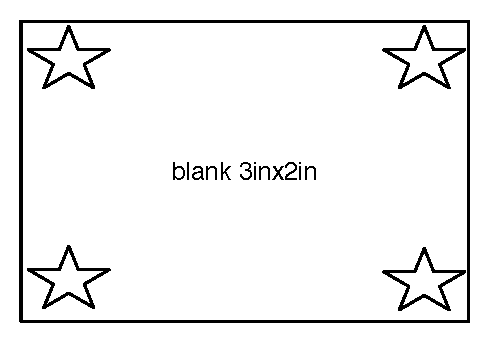
\includegraphics{figs/blank-3-2.eps}}
 \hspace{.01in}
 \subfloat[\ix]{
  \label{fig:pareto-eff:ix}
  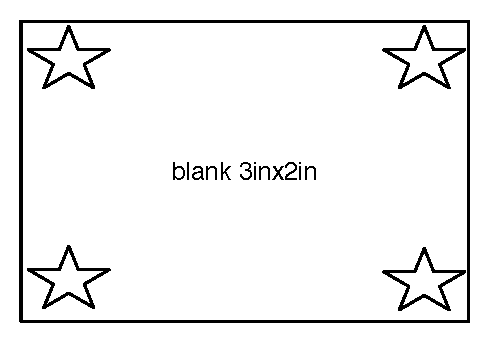
\includegraphics{figs/blank-3-2.eps}}

\caption{Pareto Efficiency measuring energy-efficiency as a function of throughput.}
\label{fig:pareto-eff}
\end{figure*}



Fig.~\ref{fig:pareto-eff} quantifies the tradeoff in terms of
energy-efficiency for two different operating systems, Linux 3.16.1
and \ix.  In these graphs, each black curve represents the energy
spent by the CPU, as measured by Intel RAPL~\cite{intel:rapl}, as a
function of the application load, for a given static configuration.  A
static configuration is determined by a number of execution threads
(from one to 16) and the CPU frequency of the socket (from 1.2 Ghz to
2.4Ghz, as well as Turbo mode).  The application is memcache, the load
generator mutilate~\cite{url:mutilate} and the workload is
USR~\cite{Atikoglu:2012:WAL}.  We only report results where the
application meets a service-level agreement of 500\microsecond
measured at the 99th percentile at the client. See
\S\ref{sec:eval:setup} for details on the experimental methodology and
setup.

In Fig.~\ref{fig:pareto-eff:linux} and Fig.~\ref{fig:pareto-eff:ix},
the red curve corresponds to the Pareto-optimal energy consumed for
any given application load.  The concept of Pareto efficiency (or
optimality) is broadly used in finance, life-sciences, and engeenering
to determine the optimal allocation of resources that maximizes a
particular objective function~\cite{wikipedia-pareto}.  The approach
is first useful to rule out the combinations that are suboptimal under
particular circumstances.  Fig.~\ref{fig:pareto-eff:linux} and
Fig.~\ref{fig:pareto-eff:ix} only shows the static configurations that
contribute at least one data point to to the Pareto-optimal curve.
There are 17 such static configurations for Linux and 21 for \ix.  To
put this in perspective, the cross-product of 16 possible number of
threads and 14 different clock rates leads to 224 distinct
configurations.  And of course, in the absence of any static
configuration tradeoff, a single configuration would suffice.

A detailed comparison of the Pareto-optimal curves of
Fig.~\ref{fig:pareto-eff:linux} and Fig.~\ref{fig:pareto-eff:ix}
further shows that the two operating systems have different
energy-efficiency characteristics.  First, Linux relies on interrupts
to save energy a low loads, resulting in a large dynamic spread for
each curve; in contrast, \ix relies on polling to deliver load
latency, resutling in flatter curves.  Consequently, there is also a
tradeoff between the two operating systems.  Indeed, Linux is more
energy-efficent than \ix with loads of less than XXX requests per
second.  Second, certain Linux configurations draw noticeably more
energy than \ix.  This is simply due to the fact that memcache
scalability bottlenecks at the application level limit the number of
useful threads to 9 on \ix but to 16 on Linux.  Third, the maximal
throughput of the both Linux and \ix noticeably exceed our previoiusly
reported results in \~cite{ix-osdi}; those are due primarily to recent
changes made to memcache to improve its horizontal scalability.  And
finally, at maximal load, \ix outperforms Linux by 2.0$\times$ while
drawing only 71\% of the energy.


\subsection{Server Consolidation}

Fig.~\ref{fig:pareto-consolidation} shows the similar Pareto
efficiency in the server consolidation scenario, which combines a
CPU-intensive background job with the same latency-sensitive memcache
workload.


\section{Control Loop}

The dataplanes are controlled by the control plane.
The control plane is a normal system daemon which has a centralized view of various exposed performance metrics of each dataplane.
Based on these metrics and a preconfigured control algorithm, it decides on the resource allocation for each dataplane.
The objective of the control plane is to assign the minimal amount of resources to each dataplane without reducing its achieved performance or compromising its expected SLA.
The SLA is expressed in terms of the tail latency.
The dataplane provides a set of metrics which are proportional to the latency of the hosted network application.
The network application latency is an end-to-end metric and as such it cannot be captured directly by the underlying operating system without prior knowledge of the application itself or its network protocol.
Since such coupling is not desired, the tail latency is calculated based on a set of metrics which can be reliably measured at the operating system level.

\subsection{Energy-optimal allocation of resources}

In this section, we describe the designed policy for achieving energy-optimal allocation of resources to dataplanes.
The initial state of the resource allocation is to dedicate a single core to the dataplane and set the CPU package at the lowest possible clock frequency.
The general strategy is simple and adheres to following pattern: to cope with increasing load, the control plane first increases the number of allocated cores, and when this number reaches a maximum value, the control plane gradually increases the clock frequency of the CPU package.
This strategy provides the closest achievable behavior to an ideal CPU whose energy consumption is linearly proportional to its utilization.

\section{Mechanisms}

The control plane uses two distinct mechanisms to control resource usage.
It can alter the number of assigned CPU cores to each dataplane.
It can modify the CPU frequency clock.

IX boots with the configured maximum number of cores.
Each core spins waiting for network activity or commands from the control plane.
Upon the reception of the respective control plane command, IX executes a blocking system call from the retiring core.
That way, Linux regains control of the core and can either schedule other processes or decide to let the core idle, depending on Linux scheduler's decisions.
The IX thread blocks on a named pipe, which can be signaled by the control plane in order to wake up the IX thread which will recover ownership of the respective core and continue its processing.
\george{reference to exokernel revokation protocol}

Additionally, the control plane is able to control the operating clock frequency of the CPU.
Linux exposes the DVFS mechanism available in modern processors through its \texttt{/sys} filesystem.
The control plane writes to specially designated files in that filesystem in order to set the operating frequency of the CPU.
Consequently, the mode of operation of this mechanism is transparent to the execution of the dataplane.
There is no need to communicate the increase or decrease of processor clock frequency to the dataplane.

TCP traffic is identified by a tuple of 4 elements: source IP, source port, destination IP, and destination port.
Modern NICs are capable to filter traffic based on these elements and direct it to specific hardware queues.
FlowDirector is an example of this technology.
We felt that this kind of fine-grained control is not necessary to achieve the goals of this paper, so we relied on a more coarse-grained technique.
The NIC computes a hash function over the elements of its packet's tuple.
An example of this hash is the RSS hash.
The Intel X520, which we used for our implementation, takes the 7 least significant bits of this hash and names them flowgroup.
There are, thus, 128 flowgroups and each one of them can be directed to one of the 16 available hardware queues.
Each flowgroup can contain an arbitrary number of TCP flows.
A TCP flow cannot change flowgroup since its tuple does not change.
Moreover, we assume that the hash function is well-designed and distributes TCP flows uniformly across the 128 available flowgroups.
These reasons are enough for our purposed to adopt the flowgroup as the unit of traffic management for our system.

Each NIC hardware queue is processed by a single CPU core.
That means that a core is responsible for processing a number of flowgroups, which are directed to the specific hardware queue.
Additionally, the system is capable of migrating on-the-fly a flowgroup between hardware queues and, thus, CPU cores.
This migration is a specially challenging task and we will explain why.
IX is designed in order to maximize the performance of TCP-based network applications.
One of its fundamental contributions is the coherence-free operation, which is achieved because IX prevents inter-core communication.
That means that each utilized data structure belongs to a single core and is only accessed by it.
Tieing data structures to each core is fine as long as you do not consider any kind of flow rebalancing.
Our major contribution is the evolution of per-core data structures to per-flowgroup ones.
Each flowgroup has its own set of data structures and IX has to make sure that only a single core accesses them at a given time.
In order to guarantee coherence-free operation we designed a handoff protocol.
The coordinator of the handoff is the control plane, which decides that it wants to migrate flowgroup 1 from core A to core B.

\george{describe handoff}


\section{Internal notes}


\subsection{ CUT from Intro}



In addition, such applications must scale in terms of bandwidth and
concurrent connection counts, and ideally solve the \emph{C10M
  problem}~\cite{theC10Mproblem}: for a given server, scale to 10
million concurrent TCP connections, saturate 10 GbE interfaces, and
deliver 10~\microsecond latency (mean), with an additional latency
jitter of not more than an extra 10~\microsecond.  Today, million+
concurrent connections are desirable in Internet-facing notification
servers~\cite{DBLP:conf/sosp/AdyaCMP11} or messaging
servers~\cite{whatsapp-2mil}. 


\begin{comment}

%%% V1

We focus here on three high-level challenges for web-scale
applications that point to the need to address energy-proportionality,
connection scalability, and quality-of-service for web-scale
applications.

First, at the highest level, web-scale applications ideally deliver
the highest possible quality of service in the most
energy-proportional manner~\cite{DBLP:journals/computer/BarrosoH07}.
In practice, these two goals are often at odds with each other:
techniques that can improve quality-of-service, and in particular
reduce end-to-end latency, often consume much more energy.  For
example, low-power states save substantial amounts of energy, at the
cost of an increased latency measured in XXX when transitioning back
into a normal operating system.

Second, the nodes of web-scale applications are often characterized by
extremely high fan-out and high fan-in requirements.  An application
server may rely on tens of thousands of downstream services, and a
downstream service may serve hundreds of thousands of
clients~\cite{missing}.  At the extreme end of the spectrum,
notification and communication services must scale to the hundreds of
millions of Internet clients~\cite{DBLP:conf/sosp/AdyaCMP11}.
Unfortunately, existing implementations of the TCP/IP networking stack
in current systems were never designed to scale to such sizes.  As a
consequence, Facebook pragmatically chose to forgo the TCP protocol in
favor of connection-less UDP datagrams~\cite{nishtala2013scaling} for
its memcached implementation.  WhatsApp put significant engineering
efforts to tun FreeBSD to scale to 2 million concurrent
connections~\cite{whatsapp-2mil}.

Third, these high fan-in and fan-out applications suffer from the
\emph{long tail} problem, with the latency of the application
determined by the latency of slowest-responding
node~\cite{DBLP:journals/cacm/DeanB13}.  To lessen the impact of the
long tail, datacenter operators often overprovision servers to ensure
that they can operate at low utilization.

Collectively, the second and third challenge have been proposed as the
\emph{C10M problem}~\cite{theC10Mproblem}: for a given server, scale
to 10 million concurrent TCP connections, saturate 10 GbE interfaces,
and deliver 10~\microsecond latency (mean), with an additional latency
jitter of not more than an extra 10~\microsecond.  The conventional
wisdom is that such a solution must bypass the operating system
entirely.  For example, mTCP~\cite{jeong2014mtcp} is a user-level TCP
stack with the highest known scalability for short-lived connections.

\end{comment}


\subsection{Stuff to cite somehow}
\begin{itemize}


\item DPDK
\item IXGBE
\item some kind of user-mode zero-copy network driver, but I think it is proprietary. \url{http://www.ntop.org/products/pf_ring/}
\item same for FreeBSD \url{https://www.usenix.org/system/files/conference/atc12/atc12-final186.pdf}
\item mTCP - highly scalable userspace multicore TCP kernel~\cite{jeong2014mtcp}.  Site at \url{http://shader.kaist.edu/mtcp/}
\item Megapipe~\cite{han2012megapipe},
\item Affinity-accept~\cite{DBLP:conf/eurosys/PesterevSZM12}
\item Netmap~\cite{rizzo2012netmap}.
\item SO\_RESUEPORT (socket option).  
\item What's App 2milion socket post~\cite{whatsapp-2mil}
\item Dune~\cite{belay2012dune} ...
\end{itemize}

\subsection{Names and Concepts of IX}

\begin{itemize}
\item {\bf cpu}. A hardware thread, labelled x/y with x the core and y the HT
\end{itemize}


\subsection{To put in related work}

\paragraph*{Exokernel}   Exokernels~\cite{DBLP:conf/sosp/EnglerKO95} safely expose hardware to library operating systems.  We propose


\paragraph*{Akkaris}.  
Akkaris~\cite{peter2013arrakis} is the closest system.  It is
apparently built on the barrelfish multikernel~\cite{DBLP:conf/sosp/BaumannBDHIPRSS09} and uses VT-x
like Dune~\cite{belay2012dune}.

\paragraph*{Megapipe} 
Megapipe~\cite{han2012megapipe} proposes a high-performance socket
alternative for TCP/IP based applications for scalable network
applications.  Our API is inspired by it. This is similar to
Netmap~\cite{rizzo2012netmap}, which also ping shared buffers, but is
focused on libpcap applications.


\paragraph{mTCP}

MTCP is a user-level stakc (NSDI 2012) that outperform Megapipe and
Linux (w/ SO\_REUSEPORT) by large factors.  The design calls for a
userlevel TCP stack that runs in the same address space as the
application. The threading model calls for a 1:1 correspondance
between application threads and TCP threads, ideally running on the
two different hyperthreads of the same core.  This gives TCP threads
to run timers with high precision.  To offset the high cost of IPC,
mTCP relies on extensive batching of commands before waking the
distinct thread.  There is no protection between application and TCP
thread; a malicious (or owned) application can easily corrupt the TCP
protocol blocks and header space.  mTCP is built on top of the PSIO
engin, which provides an event-driven packet IO interface.

In constast, IX runs the TCP stack (in kernel model) and the
application on the same threads of control; an IX application can
therefore take advantage of all hyperthreads of the CPU (instead of
only half).  Furthermore, IX runs without any locks, lock-free data
structures, or atomic instructions, whereas mTCP relies on lock-free
data structures (which themsevles require atomic instructions).

mTCP does not expose the dual-thread model directly to
applications. Instead, it hides it behind a nearly-identical POSIX
variant (epoll --> mepoll).  IX exposes an event-driven API directly
to applications, via the libevent framework.

MTCP has some great design ideas that IX could/should leverage:

\begin{itemize}

\item Efficient timer management for high-socket count.  One bucket
  per remaining milisecond for near-term events, and an ordered list
  for longer-term events (TCP cleanup events).

\item They claim optimization for
short-lived connections, including the prioritization of SYN and ACK
packets on TX (which seems like a hack)

\end{itemize}

The evaluation of MTCP includes micro-benchmarks as well as basic
applications (ab + lighttpd, SSLshader).  Fig 7 shows the connection
setup/taredown throughput based on the number of cores, showing linear
speedup up to the measured 8 cores.  At 8 cores, they can setup, send
a 64B message and close a connection 150,000 times per second, using 8
cores (i.e. 16 threads).  They can actually accept/close 300,000
connections per second (Fig 8).

SSLsharer runs with up to 16K connections; they measure median and 95
percentile latency for response time.

They use the Jain index on a benchmark that downloads a 10MiB file
repeatedely across 8K connections to measure fairness.  8K is a small
number of connections.  Table 4 looks at the connection count and
thrhougput of WebReplay across 4x10GbE connections.  The workload
creates up to 15K connections per second and has up to 25k concurrent
connection (the text also mentions having up to 270,000 conurrent
connections).




\paragraph*{Kernel-bypass approaches}  Solarflare Openonload~\cite{openonload}, ...

\paragraph*{Containers}  Linux containers, BSD jail, ...


\paragraph*{Application-specific kernels}  
Exokernels had a bunch of them.
SplashOS~\cite{DBLP:journals/tocs/BugnionDGR97} proposed this in the
context of hypervisors (Disco).
Libra~\cite{DBLP:conf/vee/AmmonsABSGKKRHW07} was a JVM that ran
directly on top of Xen.  It Relied on a separate Linux VM to provide
networking and storage (like Azul).  The
Unikernel~\cite{DBLP:conf/asplos/MadhavapeddyMRSSGSHC13} (ASPLOS 13)
lays out the case for BaremetalOS because it lays out the case for
single app operating systems.  The Unikernel ported the Ocaml runtime
to run on top of Xen hypervisor (like libra).  Actually makes a case
for reduced latency jitter, at least in terms of thread scheduling -
I/O performance basically sucks though because still not taking
advantage of HW (uses Xen PV-NIC).

\section{Techniques and Concepts}

\paragraph*{The C10M problem} As stated by Robert Graham(?)~\cite{theC10Mproblem}.


\paragraph*{Scheduler activations} 
If apps are able to yield cores, and if apps are able to
asynchronously take advantage of new cores, scheduler
activations~\cite{DBLP:journals/tocs/AndersonBLL92} seem like a
perfect mechanism to make those cores available to other processes. 
The idea never really made it into POSIX, but we can use here because the API is different. 

\paragraph*{Ballooning}
Ballooing was introduced for memory
management~\cite{DBLP:conf/osdi/Waldspurger02}.  The balloon keeps
track of the amount of relinquished resources.  CPU ballooning could
be used to (i) start a max core pool, and (ii) dynamically resize it
according to the SLA and the global load.

\paragraph*{Virtual memory performance}  
Direct segment mapping~\cite{DBLP:conf/isca/BasuGCHS13} proposes to
replace the traditional TLB with a dedicated direct segment.
Drepper~\cite{DBLP:journals/queue/Drepper08} measured additional cost
of running workloads in virtualized domains due to two-dimensional
page walking.

\paragraph*{Latency distribution}  
Dean and Barroso~\cite{DBLP:journals/cacm/DeanB13} describe the
problems associated with tail latency in web-scale services.
Dynamo~\cite{DBLP:conf/sosp/DeCandiaHJKLPSVV07} talked about the
importance to evaluate key-value stores based on their 99.9\% latency.


\paragraph*{Commutativity and scalability} 
The scalable commutativy rule~\cite{DBLP:conf/sosp/ClementsKZMK13}
states that only commutative APIs can be implemented in a truly
scalable manner; our API and our implementation should support that.
RadixVM~\cite{DBLP:conf/eurosys/ClementsKZ13} provides scalable
address spaces for multithreaded applications; we address this as well.

\paragraph{The case against user-level networking}
Margo's original paper (same title)~\cite{magoutis2004case}

\paragraph*{Latency measurements}  

\section{Workloads}

\paragraph*{Memcached} 
Scaling memcached at Facebook~\cite{nishtala2013scaling} required
unnatural tricks such as relying on UDP and on in-network connection
proxies to compensate for the lack of scoket scalability of Linux.

Memcached is so important that folks are prototyping it in
FPGA~\cite{DBLP:conf/fpga/ChalamalasettiLWARM13}.  The authors's main evaluation is
that they can get comparable performance to an industry server with
10x the Performance/Watt, measured in KOPS/S/Watt (Table 3. memcached
``gets'' with 128B size data). To beat their numbers, we need to beat
30 Kops/sec/W to win.  Can we?  The comparison is a case of hardware
specialization vs. software specialization (of the OS).



\paragraph*{ngnx}

\bibliographystyle{plain}%abbrvnat}
\bibliography{../common/gen-abbrev,dblp,../common/gscholar,../common/misc}

\end{document}







